\chapter{Services}\label{ch:services}


\section{Traefik Edge Router}\label{sec:traefik}

\begin{figure}[ht]
    \centering
    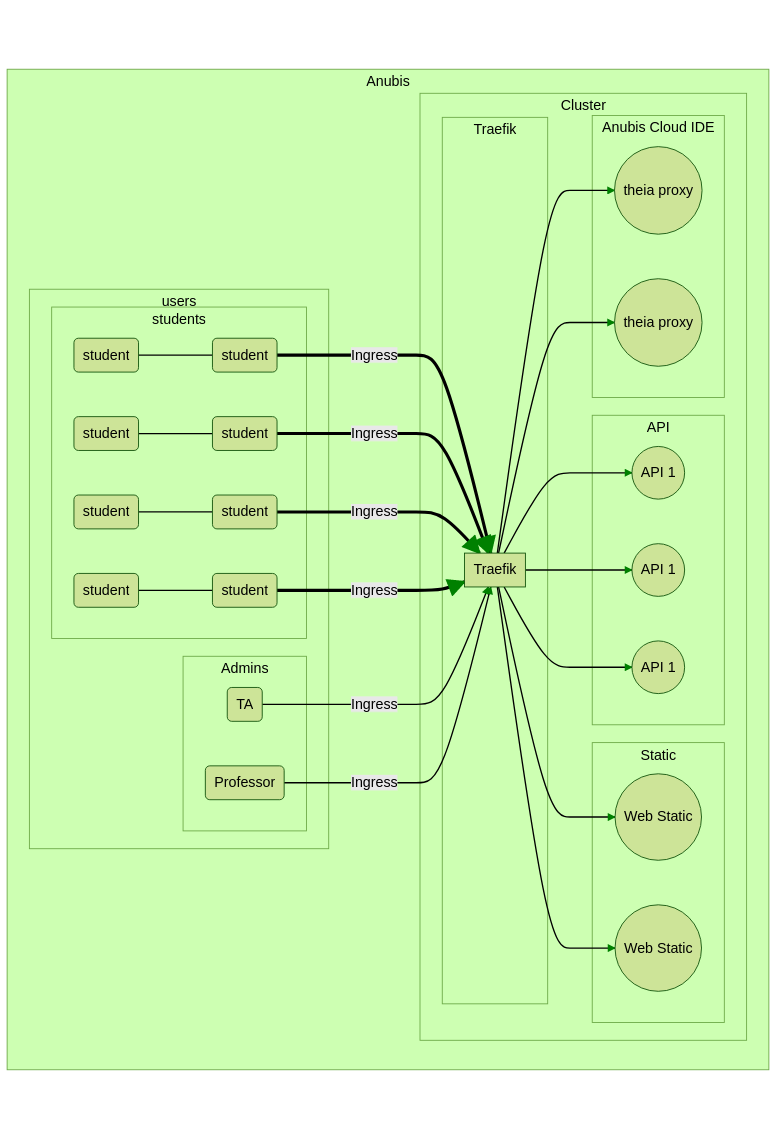
\includegraphics[width=0.5\textwidth]{figures/traefik.mmd}
    \caption{Traefik Traffic in Anubis\label{fig:traefik}}
\end{figure}

For our edge router, we use traefik~\fref{fig:traefik}.
Traefik will be what actually listens on the servers external ports.
All external traffic will be routed through Traefik.
Above all else, we will be using Traefik's powerful routing features to handle the ingress of requests.

Traefik lets us do some spicy and powerful stuff.
We can route requests to different services based off predefined rules,
and even change requests as they pass through.

Among other things, the routing rules make it so that we can have
both the static store and api on the same domain.
The rules are set up such that every request that
starts with a path of \textit{anubis.osiris.services/api/*} goes to the api~\fref{sec:api} service.
All other requests \textit{anubis.osiris.services/*} are routed to the web static~\fref{sec:web} service.

In addition to having the web static~\fref{sec:web} and the anubis api~\fref{sec:api} services on
the same domain, we can add routing rules for the theia-proxy~\fref{sec:theia-proxy} service.
Anything that is \textit{ide.anubis.osiris.service/*} will be routed to the theia-proxy service~\fref{sec:theia-proxy}.

By leveraging these features of Traefik, we can make it appear that
the services work different when being accessed externally.


\section{Anubis API}\label{sec:api}

The API is the backbone of Anubis.
It is where most of the heavy lifting is done.
The service relies on both the cache~\fref{sec:caching} and mariadb data
stores~\fref{sec:data-stores} to maintain state.

The Anubis API is itself nothing more than a simple \href{https://flask.palletsprojects.com/en/2.0.x/}{Flask} app.
As of version \textit{v3.1.16} it is about 25,000 lines of python.

\subsection{Zones}\label{subsec:api-zones}

The API is split into two distinct, and uniquely treated zones.
There is a public and a admin zone.
All endpoints for Anubis fall within one of these zones.
In the source code for Anubis, the views for these zones exist
in seperate public and admin python modules.

All public view endpoints will start with the url \textit{anubis.osiris.services/api/public/*}.
Similarly, the admin view endpoints will start with \textit{anubis.osiris.services/api/admin/*}.

\subsection{Public Zone}\label{subsec:api-public-zone}
The majority of the public API does require authentication.
This is mostly handled by the \textit{@require\_auth} decorator applied to the view function.
Additional checks will be done to verify that the resource, or calculation being requested are
something the requestor (the user making the request) is authorized to see.
The distinction must be made that public here means that it is public to users.
Students that open Anubis in a web browser and navigate through their submissions and assignments
will only be using the public API.

\subsection{Admin Zone}\label{subsec:api-admin-zone}
The admin api zone is where all the special endpoints that require higher than student level permission reside.
When a TA or Professor uses any functionality of the Admin Panel, they are using these special
admin flask views.
All of the view functions in the admin api module have decorators like \textit{@require\_admin()} or
\textit{@require\_superuser()}.
These protect the endpoints from anyone without admin permissions on at least one course.
Additional checks are then performed on each endpoint to verify that whatever resource is being requested
or modified is allowed by the current user.

\subsubsection{Course Context}\label{subsubsec:course-context}
Most view functions for the admin api require a \textit{course context} set in the cookie of the request.
When multi-course management was added to Anubis, most all the view functions for the admin api
needed to be made \textit{"course aware"}.
What that means is that there needed to be a check that the user making the request is an admin \textit{and} is
an admin for the course that that resource resides under.

\subsection{Health Checks}\label{subsec:api-health-checks}
There are very simplistic health checks in the api that make debugging issues much easier.
The endpoint \textit{anubis.osiris.services/} will run the following view function:

\begin{minted}{python}
    @app.route("/")
    def index():
        Config.query.all()
        cache_health()
        return "Healthy"
\end{minted}

The view checks that the database~\fref{sec:mariadb} is accessible by running a query, then calls a function that relies on the
redis cache~\fref{sec:caching}.
While this view function may be simple, it is quite effective.
Most of the incidents of degraded service or downtime come down to either the database or cache being temporary
unavailable.

\subsection{Responsibilities}\label{subsec:api-responsibilities}

The Anubis API is responsible for handling most basic
IO, and state managing that happens on the cluster.
Some of this includes:

\begin{itemize}
    \item Authenticating users
    \item Providing Class, Assignment, and Submission data to the frontend
    \item Handling github webhooks
    \item Handling reports from the submission pipeline cluster
    \item Handling regrade requests
    \item Initializing new IDE sessions
\end{itemize}

\subsection{Authentication}\label{subsec:api-authentication}

To authenticate with the api, a token is required.
The only way to get one of these tokens is through NYU Single Sign On.
By doing this, we are outsourcing our authentication.
This saves a lot of headaches while being arguably more secure than if we rolled our own.

All of this is about 20 lines on our end.
All that is necessary are some keys from NYU IT.


\section{Anubis Web Static}\label{sec:web}

\begin{figure}[ht]
    \centering
    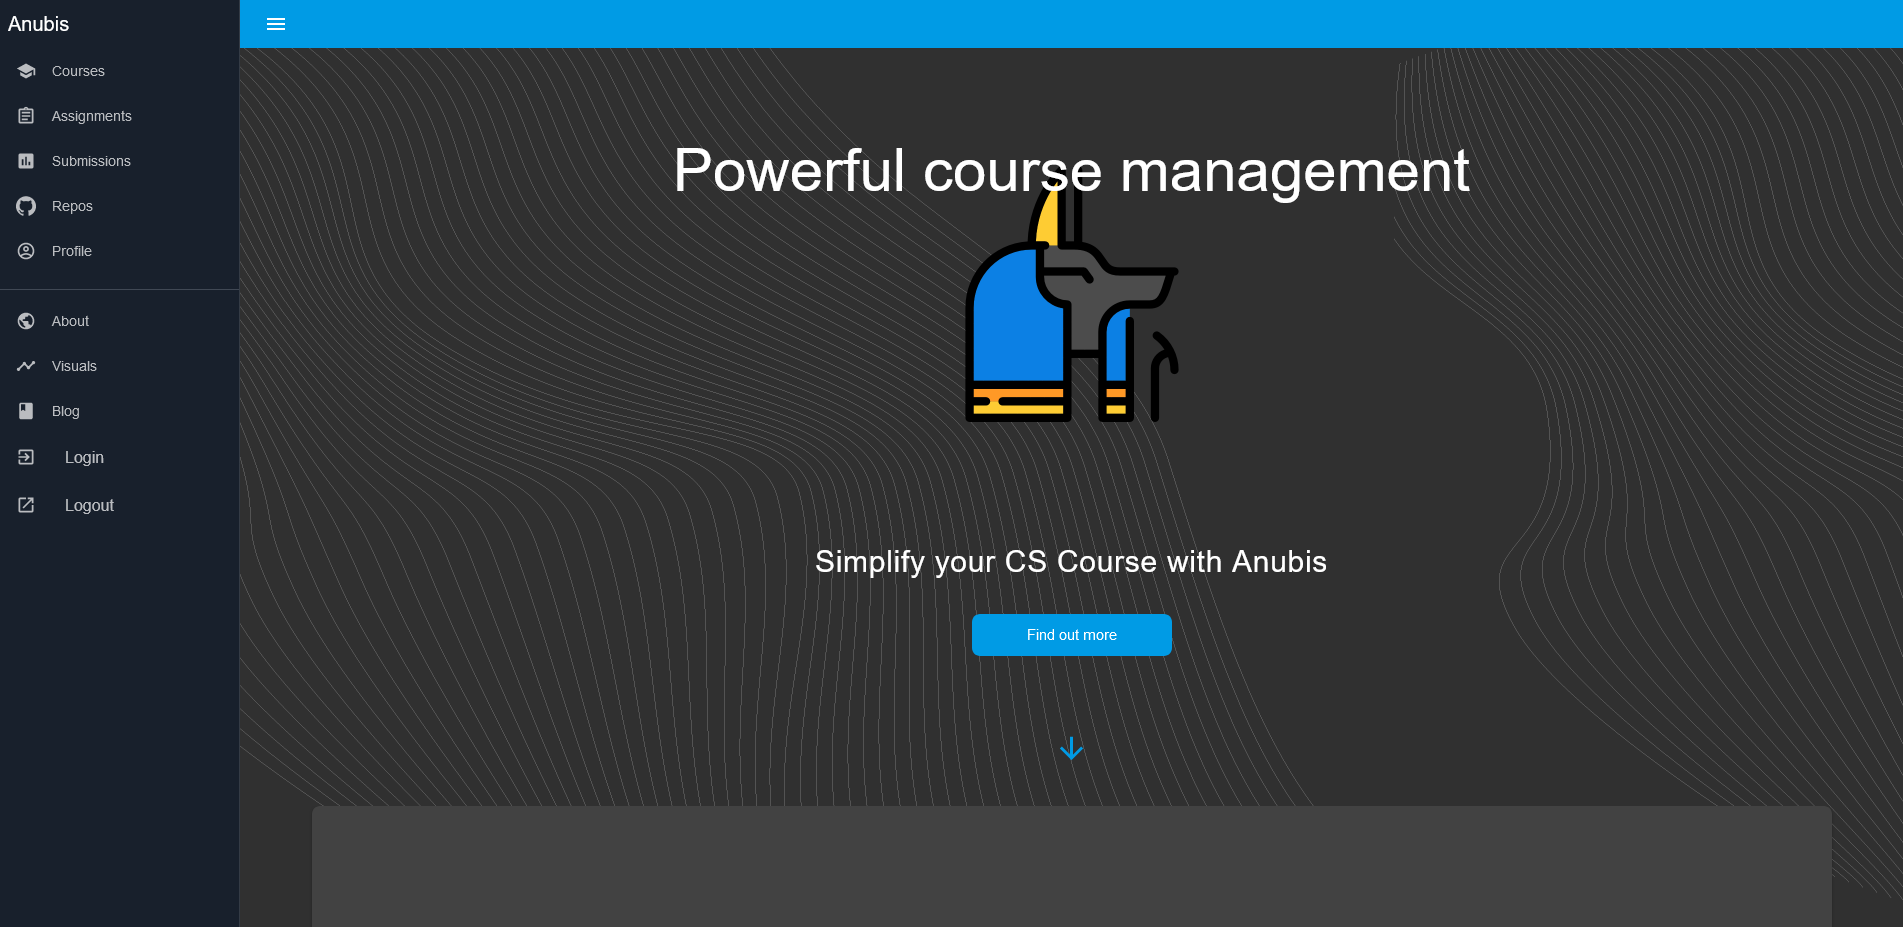
\includegraphics[width=0.75\textwidth]{figures/anubis-frontend}
    \caption{Anubis Web Frontend\label{fig:web-frontend}}
\end{figure}

The web static service is nothing more than a simple static http webserver.
There are no moving parts that are necessary for this service.
Only the compiled reactjs, html and css files are found in this service.
One thing of note that is not in this service are most images.
The only images that are in this web static image are the logo favicons
and some others.
The majority of images that are on the frontend (through the blog or assignment questions and whatnot)
are saved in the database and accessed through the api~\fref{sec:api}.

The frontend is designed to be a simple reflection of the backend data.
Once authenticated, users will be able to see the classes they are a part of,
current and past assignments, and all their submissions.
With few exceptions, the frontend is a near one to one translation of the API's data models.
Most pages will have a corresponding API endpoint.
The data shown on that page will be in exactly the form of the API response.


\section{Anubis Theia Proxy}\label{sec:theia-proxy}

The purpose of the the theia-proxy service it to route and forward student requests
to the appropriate Cloud IDE~\ref{ch:cloud_ides} instances.
Internals of this service are described in section~\ref{subsec:balancing-network-traffic}

\section{Reaper CronJob}\label{sec:reaper}

Many of the resources that Anubis allocates within the cluster are shortlived. The Cloud IDE, and Submission Pipeline
pods are the most fluid of all.
The Cloud IDEs will be created and destroyed at the behest of students.
The Submission Pipeline pods rarely last for more than a few minutes. 
For these reasons Anubis needs a frequent recurring job that keeps resources in check.
This is where the reaper job comes in. 

It compares the resources that are suppose to be allocated according to 
the database, and the resources that are actually allocated in the cluster. 
If there are IDE or Submission Pipeline resources that are allocated that 
cannot be accounted for, or should be deleted, the reaper will schedule
them for deletion.

\subsection{Reaping IDE Resources}\label{subsec:reaping-ide-resources}

When an IDE is created by a user, there is a record of the session added to the database.
With this table of records, the reaper can pull all the IDE resources that should exist.
The reaper can then pull the IDE resources that do exist from the Kubernetes api.

Comparing these two sets there may be resources that should not exist that do, or
resources that should exist that do not.
The reaper will delete resources that should be deleted or mark sessions as ended
if the resources do not exist.

There is also a hard 6 hour limit on Anubis Cloud IDEs.
Without this limit, many students would create a Cloud IDE and just forget about it.
Obviously having these resources outstanding would be an expensive problem for Anubis to have.
The reaper handles this situation by checking for active IDEs that have reached that 6 hour limit,
and schedules the resources for deletion.

In an interesting experiment in human behavior, we can plot the cumulative duration (in minutes) of
Cloud IDEs from the final exam from CS-UY 3224's fall 2020 semester~\ref{fig:theia3}.
About 60\% of all IDE sessions reached the 6 hour limit.

\begin{figure}[ht]
    \centering
    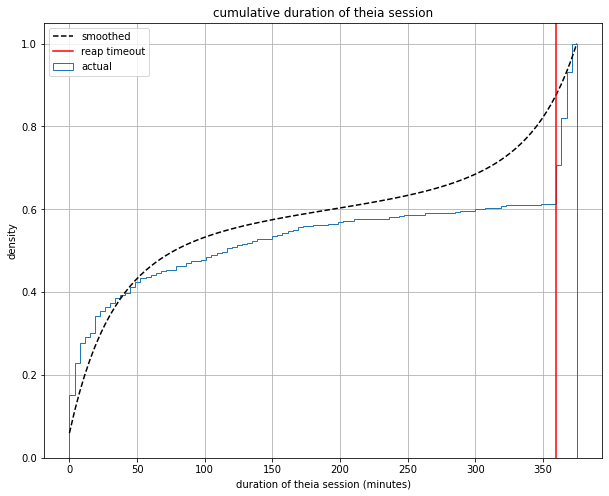
\includegraphics[width=0.5\textwidth]{figures/theia3}
    \caption{Cumlative Duration of a Theia Session\label{fig:theia3}}
\end{figure}

\subsection{Reaping Submission Pipeline Resources}\label{subsec:reaping-submission-pipeline-resources}

Submission Pipelines are run as Kubernetes batch jobs.
Batch jobs are not automatically removed (at least not without enabling
\href{https://kubernetes.io/docs/concepts/workloads/controllers/ttlafterfinished/}{ttl-controllers}).
Finished Submission Pipeline jobs are unnecessary resources.

For this reason, the reaper job will also schedule all finished and successful Submission Pipeline batch jobs
for deleteion.
Pipeline jobs that failed for whatever reason are not deleted.
This is purposeful in design so that if there is an issue with a pipeline,
there are logs that can be examined.

\subsection{Searching and Fixing Broken Submissions}\label{subsec:reaping-fixing}

The last main responsibility of the reaper is fixing broken submissions.
Anubis is what is called an \href{https://en.wikipedia.org/wiki/Eventual_consistency}{Eventually Consistent}
system.
That means that there is a certain tollerance of short term inconsistency that is expected
and handled by the system.
The place that many of these inconsistencies are remedied are in the reaper cron.

The reaper cron searches recent submissions for common signs of breakage.
These breakages could be inconsitentcies that were caused by a failed or stalled Submission Pipeline
for example.
Depending on the issue, the reaper may be able to fix or not.
For issues that cannot be fixed by the reaper, the submission is marked as broken.

Often if a student complains about some kind of inconsistency, the problem is fixed
before an Anubis admin can inspect it.
The reaper has saved countless hours for students and staff alike.

\section{RPC in Anubis}\label{sec:rpc-in-anubis}

Remote Procedual Calls are common place is many distributed systems.
Anubis relies on them quite heavily.
Many workflows in Anubis push work to RPC job queues through using the
\href{https://python-rq.org}{python-rq} library.

These calculations happen asyncronusly in worker deployments on the cluster.
RPC worker pods have additional \href{https://kubernetes.io/docs/reference/access-authn-authz/rbac/}{RBAC}
permissions that the api does not have.
These permissions enable these worker instances to interface with the kubernetes api in ways
that the api cannot.
The RPC workers can create and destroy Cloud IDE~\ref{ch:cloud-ides}
and Submission Pipeline~\fref{sec:submission-pipelines} resources in the cluster.

Jobs are organized into separate queues depending on the subject of the job.
To learn more behind the reasoning for this separation, check out the
\href{Spring 2021 Midterm Retro}{https://anubis.osiris.services/blog/midterm-retro}
blog post.

\subsection{Regrade RPC}\label{subsec:regrade-rpc}

Submission Pipeline create and or regrade jobs end up in the regrade queue.
The main reason this exists as its own queue is for bulk regrades.
When running a bulk regrade on an assignment there may be a surge of thousands of
jobs enqueued into the rpc queue (one for each submission).
To avoid a bulk regrade surge draining jobs triggered by student from resources,
this exists as its own queue

\subsection{Theia RPC}\label{subsec:theia-rpc}

All jobs that have to do with the Anubis Cloud IDEs~\ref{ch:cloud-ides} end up in the theia rpc queue.
When students click the button to launch, or to stop a Cloud IDE a job is enqueued to create or destroy 
the resources on the cluster.

For the deletion of IDE resources, the stop of the session appears to be immediate.
The resources are marked as deleted in the 

\subsection{Default RPC}\label{subsec:default-rpc}

Every job that is not a submission regrade or for a Cloud IDE makes its way to the default queue.
Some of these jobs include the generation of visual data (either in raw form or image files) and
autograding results.